%\documentclass[aspectratio=169]{beamer}
\documentclass{beamer}

% ── Theme & colours ────────────────────────────────────────────────────────────
\usetheme{Madrid}
\usecolortheme{default}

\usepackage[english]{babel}
\usepackage[T1]{fontenc}
\setbeamersize{text margin left=0.5cm,text margin right=0.5cm}

\definecolor{darkblue}{RGB}{30,70,120}
\definecolor{myblue}{RGB}{46,134,171}
\definecolor{myorange}{RGB}{247,127,0}
\definecolor{mygreen}{RGB}{76,175,80}
\definecolor{myred}{RGB}{214,40,40}
\definecolor{lightgray}{RGB}{240,244,248}
\definecolor{mypurple}{RGB}{120,50,160}

\setbeamercolor{palette primary}{bg=darkblue,fg=white}
\setbeamercolor{palette secondary}{bg=myblue,fg=white}
\setbeamercolor{palette tertiary}{bg=darkblue,fg=white}
\setbeamercolor{palette quaternary}{bg=darkblue,fg=white}
\setbeamercolor{structure}{fg=darkblue}
\setbeamercolor{section in toc}{fg=darkblue}
\setbeamercolor{alerted text}{fg=myorange}
\setbeamercolor{block title}{bg=darkblue,fg=white}
\setbeamercolor{block body}{bg=lightgray,fg=black}
\setbeamercolor{block title alerted}{bg=myorange,fg=white}
\setbeamercolor{block body alerted}{bg=lightgray,fg=black}
\setbeamercolor{block title example}{bg=mygreen!70!black,fg=white}
\setbeamercolor{block body example}{bg=lightgray,fg=black}

\setbeamertemplate{navigation symbols}{}
\setbeamertemplate{caption}[numbered]

% Tighten block inner vertical padding (less wasted margin around block text)
\addtobeamertemplate{block begin}{}{\vspace{0.2em}}
\addtobeamertemplate{block end}{\vspace{0.2em}}{}
\addtobeamertemplate{block alerted begin}{}{\vspace{0.2em}}
\addtobeamertemplate{block alerted end}{\vspace{0.2em}}{}
\addtobeamertemplate{block example begin}{}{\vspace{0.2em}}
\addtobeamertemplate{block example end}{\vspace{0.2em}}{}

% ── Packages ───────────────────────────────────────────────────────────────────
\usepackage{amsmath, amssymb}
\usepackage{graphicx}
\usepackage{booktabs}
\usepackage{colortbl}
\usepackage{multirow}
\usepackage{tikz}
\usetikzlibrary{arrows.meta, positioning, calc, fit, backgrounds}
\usepackage{pgfplots}
\pgfplotsset{compat=1.18}
\usepgfplotslibrary{groupplots}

% ── Macros ─────────────────────────────────────────────────────────────────────
\newcommand{\piTheta}{\pi_\theta}
\newcommand{\Ahat}{\hat{A}_t}
\newcommand{\ppRatio}{\varrho_t}
\newcommand{\highlight}[1]{\textcolor{myorange}{\textbf{#1}}}
\newcommand{\good}[1]{\textcolor{mygreen!60!black}{\textbf{#1}}}
\newcommand{\bad}[1]{\textcolor{myred}{\textbf{#1}}}

% ── TikZ styles reused across frames ───────────────────────────────────────────
\tikzset{
  bxB/.style={draw=darkblue,    fill=darkblue!15,       rounded corners=3pt,
              minimum width=#1, minimum height=0.78cm,   align=center,
              font=\scriptsize, line width=1pt},
  bxO/.style={draw=myorange!80!black, fill=myorange!15, rounded corners=3pt,
              minimum width=#1, minimum height=0.78cm,   align=center,
              font=\scriptsize, line width=1pt},
  bxG/.style={draw=mygreen!60!black,  fill=mygreen!15,  rounded corners=3pt,
              minimum width=#1, minimum height=0.78cm,   align=center,
              font=\scriptsize, line width=1pt},
  bxR/.style={draw=myred!80!black,    fill=myred!15,    rounded corners=3pt,
              minimum width=#1, minimum height=0.78cm,   align=center,
              font=\scriptsize, line width=1pt},
  bxP/.style={draw=mypurple!70!black, fill=mypurple!15, rounded corners=3pt,
              minimum width=#1, minimum height=0.78cm,   align=center,
              font=\scriptsize, line width=1pt},
  bxGR/.style={draw=gray!60, fill=gray!10, rounded corners=3pt,
               minimum width=#1, minimum height=0.78cm,  align=center,
               font=\scriptsize, line width=1pt},
  arr/.style={-{Stealth[length=5pt]}, thick},
}

% ── Title ──────────────────────────────────────────────────────────────────────
\title[LG-SA for CVRP]{%
  Learning-Guided Simulated Annealing\\
  for the Capacitated Vehicle Routing Problem}
\subtitle{ICAPS 2026}
\author[J. Andretti]{Jules Andretti, Jérémie Cabessa, Yann Strozecki}
\institute[UVSQ]{David Laboratory, UVSQ -- Université Paris-Saclay}
\date{2026}

% ══════════════════════════════════════════════════════════════════════════════
\begin{document}
% ══════════════════════════════════════════════════════════════════════════════

\begin{frame}\titlepage\end{frame}

% ══════════════════════════════════════════════════════════════════════════════
\section{Background}
% ══════════════════════════════════════════════════════════════════════════════

% ──────────────────────────────────────────────────────────────────────────────
% Slide — CVRP
% Say: CVRP is a fundamental routing problem. Given a depot and customers
% with demands, find routes for a fleet of capacitated vehicles that visit
% every customer and minimize total travel distance.
% Note: point to the figure — depot is the star, customers are circles
% (size = demand). Right panel shows a feasible solution with 4 routes.
% ──────────────────────────────────────────────────────────────────────────────
\begin{frame}{The Capacitated Vehicle Routing Problem (CVRP)}
  \begin{columns}[T]
    \column{0.48\textwidth}
    \begin{center}
      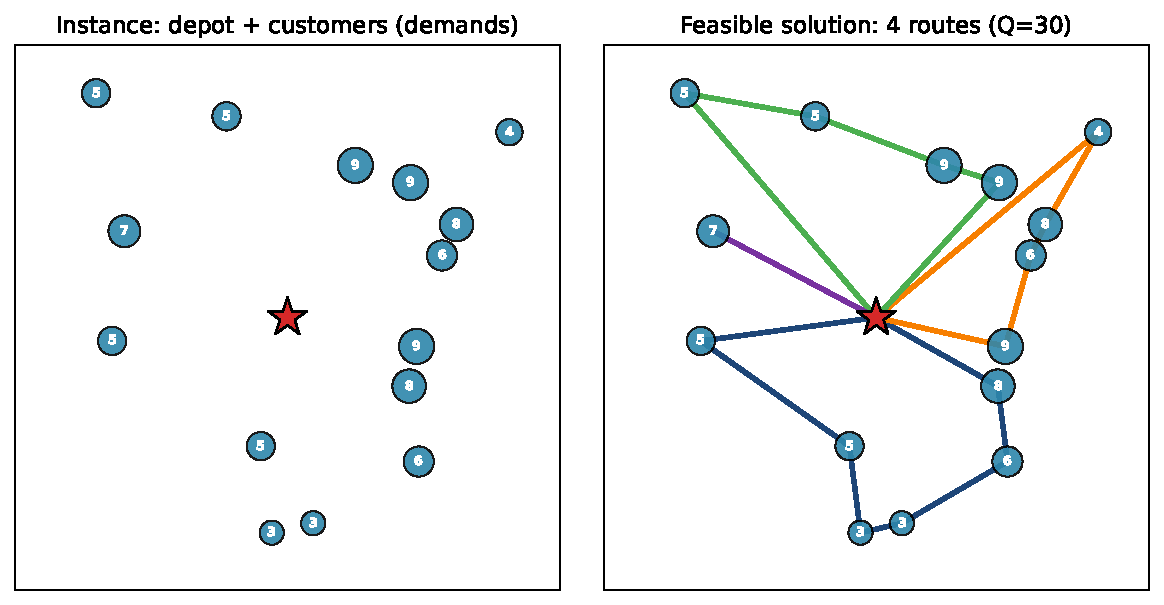
\includegraphics[width=\textwidth]{figures/cvrp_example.pdf}
    \end{center}

    \column{0.49\textwidth}
    % Say: One objective — minimize total travel distance.
    \begin{block}{Objective}
      \small Minimize total travel distance
      \[
        \min \sum_{(i,j)\in E} c_{ij}\, x_{ij}
      \]
    \end{block}
    % Say: Two hard constraints — every customer served exactly once, and
    % total demand on each route must not exceed vehicle capacity Q.
    \begin{block}{Constraints}
      \small
      \begin{itemize}
        \item $N$ customers, each visited exactly once
        \item Route load $\leq Q$ (vehicle capacity)
      \end{itemize}
    \end{block}
  \end{columns}
\end{frame}

% ──────────────────────────────────────────────────────────────────────────────
% Slide — Our Goal (SIMPLIFIED + visual)
% Say (oral): improvement metaheuristics like SA are great on CVRP — robust,
% simple, and they handle the hard capacity constraints naturally. Their
% weakness: they propose moves blindly, at random, so convergence is slow.
% Our goal: replace ONLY that blind randomness with a smarter proposal —
% and keep the model TINY (a small MLP, no heavy network). This extends
% Neural SA [Correia et al., 2023] from TSP to CVRP.
% ──────────────────────────────────────────────────────────────────────────────
\begin{frame}{Our Goal: Accelerate an Improvement Metaheuristic}
  \vspace{0.2em}
  \begin{columns}[T]
    \column{0.46\textwidth}
    \begin{exampleblock}{Metaheuristics on CVRP}
      \small
      \begin{itemize}\itemsep3pt
        \item[\good{$\checkmark$}] Robust \& simple
        \item[\good{$\checkmark$}] Handle hard constraints \\(capacity) naturally
        \item[\bad{$\times$}] Moves proposed \bad{at random} \\$\Rightarrow$ blind, \bad{slow} convergence
      \end{itemize}
    \end{exampleblock}

    \column{0.52\textwidth}
    \vspace{0.4em}
    \begin{center}
    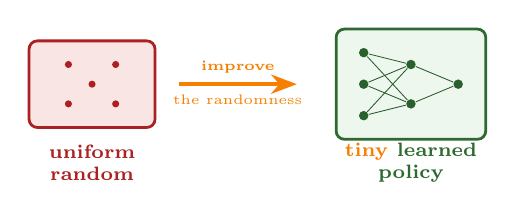
\begin{tikzpicture}[>=Stealth, font=\scriptsize]
      % ── random proposal (dice) ──────────────────────────────
      \node[draw=myred!80!black, fill=myred!12, rounded corners=3pt,
            minimum width=1.6cm, minimum height=1.1cm, line width=1pt]
        (dice) at (0,0) {};
      \foreach \p in {(-0.3,0.25),(0.3,0.25),(-0.3,-0.25),(0.3,-0.25),(0,0)}
        \fill[myred!80!black] \p circle (0.045);
      \node[font=\scriptsize\bfseries, myred!80!black, align=center]
        at (0,-1.0) {uniform\\random};

      % ── arrow ──────────────────────────────────────────────
      \draw[->, line width=1.4pt, myorange]
        (1.1,0) -- node[above, font=\tiny\bfseries, myorange]{improve}
                   node[below, font=\tiny]{the randomness} (2.6,0);

      % ── tiny policy (small MLP) ─────────────────────────────
      \begin{scope}[shift={(4.05,0)}]
        \node[draw=mygreen!60!black, fill=mygreen!10, rounded corners=3pt,
              minimum width=1.9cm, minimum height=1.4cm, line width=1pt] (net) {};
        \foreach \k/\y in {1/0.4,2/0,3/-0.4} \node[circle, fill=mygreen!55!black,
              minimum size=0.12cm, inner sep=0pt] (in\k) at (-0.6,\y) {};
        \foreach \k/\y in {1/0.25,2/-0.25} \node[circle, fill=mygreen!55!black,
              minimum size=0.12cm, inner sep=0pt] (hi\k) at (0,\y) {};
        \node[circle, fill=mygreen!55!black, minimum size=0.12cm, inner sep=0pt]
              (ou) at (0.6,0) {};
        \foreach \a in {1,2,3} \foreach \b in {1,2}
          \draw[mygreen!50!black, line width=0.3pt] (in\a) -- (hi\b);
        \foreach \b in {1,2} \draw[mygreen!50!black, line width=0.3pt] (hi\b) -- (ou);
      \end{scope}
      \node[font=\scriptsize\bfseries, mygreen!60!black, align=center]
        at (4.05,-1.0) {\highlight{tiny} learned\\policy};
    \end{tikzpicture}
    \end{center}
  \end{columns}
  \vspace{0.6em}
  \begin{alertblock}{Our idea}
    \small Keep the metaheuristic --- replace \highlight{only the blind randomness}
    with a \highlight{tiny model} (small MLP, \bad{no heavy network}). \\[0.2em]
    \emph{Extends Neural SA [Correia et al., 2023] from TSP to \highlight{CVRP}.}
  \end{alertblock}
\end{frame}

% ──────────────────────────────────────────────────────────────────────────────
% Slide — Simulated Annealing (PIPELINE only)
% Say (oral, NOT on slide):
%   - The Metropolis criterion: improving moves always accepted, worsening
%     moves accepted with probability exp(-ΔC / T).
%   - The temperature T cools over time — high T explores, low T exploits.
%   - SA is classical and well understood; what we change is the proposal —
%     specifically the highlighted uniform sampling block.
% ──────────────────────────────────────────────────────────────────────────────
\begin{frame}{Simulated Annealing (SA)}
  \vspace{0.6em}
  \begin{center}
  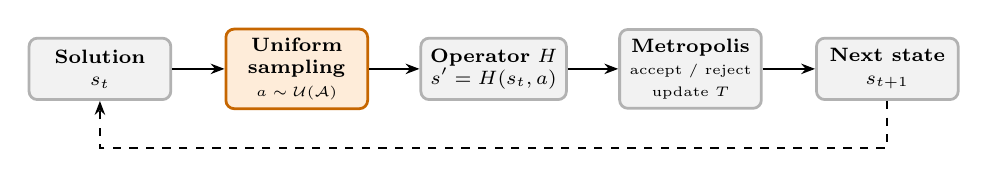
\begin{tikzpicture}[>=Stealth, thick, every node/.style={font=\footnotesize}]
    \node[bxGR=1.8cm] (s)    at (0,    0)   {\textbf{Solution}\\$s_t$};
    \node[bxO=1.8cm]  (samp) at (2.5,  0)   {\textbf{Uniform}\\\textbf{sampling}\\\tiny $a \sim \mathcal{U}(\mathcal{A})$};
    \node[bxGR=1.8cm] (H)    at (5.0,  0)   {\textbf{Operator} $H$\\$s' = H(s_t, a)$};
    \node[bxGR=1.8cm] (M)    at (7.5,  0)   {\textbf{Metropolis}\\\tiny accept / reject\\\tiny update $T$};
    \node[bxGR=1.8cm] (sn)   at (10.0, 0)   {\textbf{Next state}\\$s_{t+1}$};

    \draw[arr] (s)    -- (samp);
    \draw[arr] (samp) -- (H);
    \draw[arr] (H)    -- (M);
    \draw[arr] (M)    -- (sn);
    \draw[arr, dashed] (sn.south) -- ++(0,-0.6) -| (s.south);
  \end{tikzpicture}
  \end{center}
  \vspace{1.2em}
  % Say: This is what we keep — operator H, Metropolis. The single thing
  % we change is the proposal (uniform sampling) block, now highlighted.
  \begin{center}
    \small 
    
\begin{itemize}
\item SA proposes moves \bad{blindly}.\;
\item We change \highlight{one} block --- the proposal --- and make it \good{guided}.
\end{itemize}

  \end{center}
\end{frame}

% ══════════════════════════════════════════════════════════════════════════════
\section{Learning-Guided Simulated Annealing (LG-SA): Method}
% ══════════════════════════════════════════════════════════════════════════════

% ──────────────────────────────────────────────────────────────────────────────
% Slide — LG-SA Pipeline (same as SA pipeline + learned blocks)
% Say: Same pipeline as SA. The only change: instead of uniform sampling,
% we encode the current solution into per-node feature vectors, feed them
% to a small policy network, and sample an action (i,j) from its output.
% Note: we will detail in the next slide HOW the pair (i,j) is sampled.
% ──────────────────────────────────────────────────────────────────────────────
\begin{frame}{Learning-Guided Simulated Annealing (LG-SA)}
  \vspace{0.3em}
  \begin{center}
  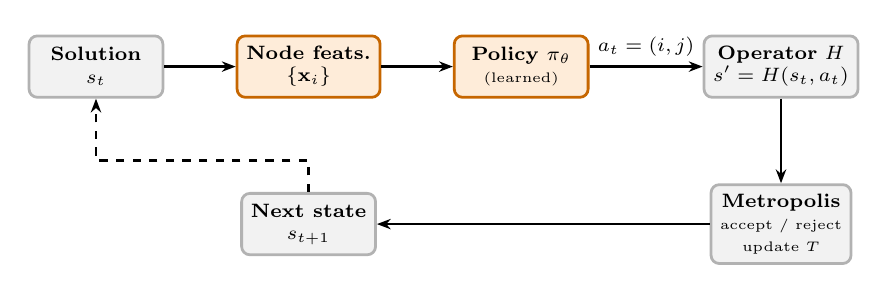
\begin{tikzpicture}[>=Stealth, thick, every node/.style={font=\footnotesize}]
    \node[bxGR=1.7cm] (s)    at (0,     0) {\textbf{Solution}\\$s_t$};
    \node[bxO=1.7cm]  (feat) at (2.7,   0) {\textbf{Node feats.}\\$\{\mathbf{x}_i\}$};
    \node[bxO=1.7cm]  (pi)   at (5.4,   0) {\textbf{Policy} $\pi_\theta$\\\tiny (learned)};
    \node[bxGR=1.7cm] (H)    at (8.7,   0) {\textbf{Operator} $H$\\$s'=H(s_t,a_t)$};

    \node[bxGR=1.7cm] (M)    at (8.7, -2.0) {\textbf{Metropolis}\\\tiny accept / reject\\\tiny update $T$};
    \node[bxGR=1.7cm] (sn)   at (2.7, -2.0) {\textbf{Next state}\\$s_{t+1}$};

    \draw[arr] (s)    -- (feat);
    \draw[arr] (feat) -- (pi);
    \draw[arr] (pi)   -- node[midway, above, font=\scriptsize] {$a_t=(i,j)$} (H);
    \draw[arr] (H.south) -- ++(0,-0.4) -| (M.north);
    \draw[arr] (M)    -- (sn);
    \draw[arr, dashed] (sn.north) -- ++(0,0.4) -| (s.south);
  \end{tikzpicture}
  \end{center}
  \vspace{0.6em}
  \begin{center}\footnotesize
    \tikz{\fill[myorange!15, draw=myorange!80!black] (0,0) rectangle (0.3,0.3);}~learned\quad
    \tikz{\fill[gray!10, draw=gray!60] (0,0) rectangle (0.3,0.3);}~classical SA
  \end{center}
\end{frame}

% ──────────────────────────────────────────────────────────────────────────────
% Slide — How the pair (i,j) is sampled (NEW)
% Say: Each node carries its own local feature vector x_i. Stage 1: each
% x_i goes through a small MLP producing a score; we softmax over all
% scores and sample the first node i. Stage 2: knowing i, we concatenate
% its features with every other node's features, run a second MLP per
% pair, softmax, sample the partner j.
% Say (oral only): we also tried a JOINT architecture — scoring every
% pair (i,j) at once. It scaled O(N^2), the tiny MLP could not rank the
% much larger pair space, and feasibility filtering became prohibitive.
% We dropped it.
% ──────────────────────────────────────────────────────────────────────────────
\begin{frame}{How the Pair $(i,j)$ is Sampled}
  \vspace{0.2em}
  \begin{center}
  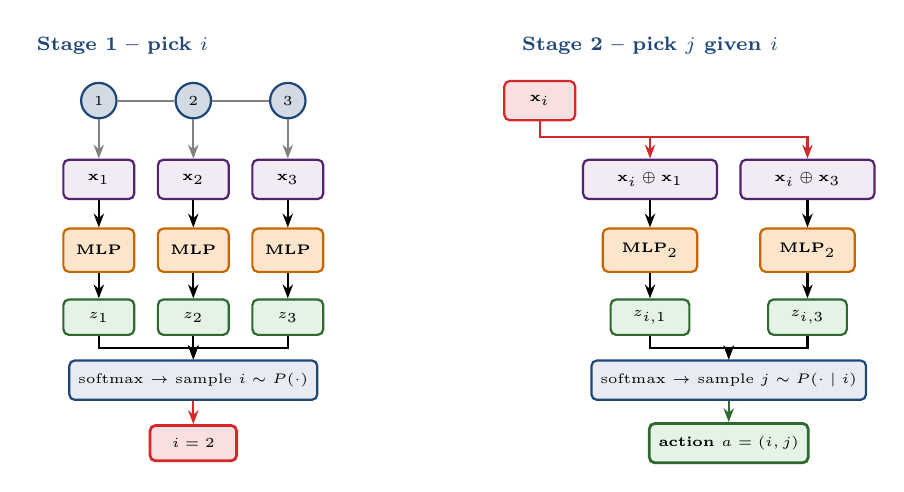
\begin{tikzpicture}[>=Stealth, thick,
      every node/.style={font=\scriptsize},
      node distance=0.6cm,
      cnode/.style={circle, draw=darkblue, fill=darkblue!20,
                    minimum size=0.45cm, inner sep=0pt, font=\tiny},
      fvec/.style={draw=mypurple!70!black, fill=mypurple!10, rounded corners=2pt,
                   minimum width=0.9cm, minimum height=0.5cm, font=\tiny},
      mlp/.style={draw=myorange!80!black, fill=myorange!20, rounded corners=2pt,
                  minimum width=0.9cm, minimum height=0.55cm, font=\tiny\bfseries},
      score/.style={draw=mygreen!60!black, fill=mygreen!15, rounded corners=2pt,
                    minimum width=0.9cm, minimum height=0.45cm, font=\tiny},
    ]

    % ─── Stage 1 (left): score every node ──────────────────────────────
    \node[font=\scriptsize\bfseries, darkblue] at (-0.3, 2.6) {Stage 1 -- pick $i$};

    % CVRP fragment (3 nodes in a route)
    \node[cnode] (n1) at (-0.6, 1.9) {1};
    \node[cnode] (n2) at (0.6,  1.9) {2};
    \node[cnode] (n3) at (1.8,  1.9) {3};
    \draw[gray, thick] (n1) -- (n2) -- (n3);

    % Feature vectors
    \node[fvec] (x1) at (-0.6, 0.9) {$\mathbf{x}_1$};
    \node[fvec] (x2) at (0.6,  0.9) {$\mathbf{x}_2$};
    \node[fvec] (x3) at (1.8,  0.9) {$\mathbf{x}_3$};
    \draw[arr, gray] (n1) -- (x1);
    \draw[arr, gray] (n2) -- (x2);
    \draw[arr, gray] (n3) -- (x3);

    % Shared MLP
    \node[mlp] (m1a) at (-0.6, 0.0) {MLP};
    \node[mlp] (m1b) at (0.6,  0.0) {MLP};
    \node[mlp] (m1c) at (1.8,  0.0) {MLP};
    \draw[arr] (x1) -- (m1a);
    \draw[arr] (x2) -- (m1b);
    \draw[arr] (x3) -- (m1c);

    % Scores
    \node[score] (z1) at (-0.6, -0.85) {$z_1$};
    \node[score] (z2) at (0.6,  -0.85) {$z_2$};
    \node[score] (z3) at (1.8,  -0.85) {$z_3$};
    \draw[arr] (m1a) -- (z1);
    \draw[arr] (m1b) -- (z2);
    \draw[arr] (m1c) -- (z3);

    % Softmax + sample
    \node[draw=darkblue, fill=darkblue!10, rounded corners=2pt,
          minimum width=2.8cm, minimum height=0.5cm, font=\tiny]
      (s1) at (0.6, -1.65) {softmax $\to$ sample $i \sim P(\cdot)$};
    \draw[arr] (z1.south) -- ++(0,-0.15) -| (s1.north);
    \draw[arr] (z2) -- (s1);
    \draw[arr] (z3.south) -- ++(0,-0.15) -| (s1.north);

    % Highlight chosen i (say i=2)
    \node[draw=myred, fill=myred!15, rounded corners=2pt, line width=1pt,
          minimum width=1.1cm, minimum height=0.45cm, font=\tiny\bfseries]
      (chosen) at (0.6, -2.45) {$i = 2$};
    \draw[arr, myred] (s1) -- (chosen);

    % ─── Stage 2 (right): pick j given i ───────────────────────────────
    \node[font=\scriptsize\bfseries, darkblue] at (6.4, 2.6) {Stage 2 -- pick $j$ given $i$};

    % Carry over x_i (selected) — drawn as anchor on top
    \node[fvec, fill=myred!15, draw=myred] (xi) at (5.0, 1.9) {$\mathbf{x}_i$};

    % Pair concatenations (with the two other nodes)
    \node[fvec, minimum width=1.7cm] (c1) at (6.4, 0.9) {$\mathbf{x}_i \oplus \mathbf{x}_1$};
    \node[fvec, minimum width=1.7cm] (c3) at (8.4, 0.9) {$\mathbf{x}_i \oplus \mathbf{x}_3$};

    \draw[arr, myred] (xi.south) -- ++(0,-0.2) -| (c1.north);
    \draw[arr, myred] (xi.south) -- ++(0,-0.2) -| (c3.north);

    % MLP2
    \node[mlp, minimum width=1.2cm] (m2a) at (6.4, 0.0) {MLP$_2$};
    \node[mlp, minimum width=1.2cm] (m2b) at (8.4, 0.0) {MLP$_2$};
    \draw[arr] (c1) -- (m2a);
    \draw[arr] (c3) -- (m2b);

    % Pair scores
    \node[score, minimum width=1.0cm] (zi1) at (6.4, -0.85) {$z_{i,1}$};
    \node[score, minimum width=1.0cm] (zi3) at (8.4, -0.85) {$z_{i,3}$};
    \draw[arr] (m2a) -- (zi1);
    \draw[arr] (m2b) -- (zi3);

    % Softmax + sample j
    \node[draw=darkblue, fill=darkblue!10, rounded corners=2pt,
          minimum width=3.0cm, minimum height=0.5cm, font=\tiny]
      (s2) at (7.4, -1.65) {softmax $\to$ sample $j \sim P(\cdot\mid i)$};
    \draw[arr] (zi1.south) -- ++(0,-0.15) -| (s2.north);
    \draw[arr] (zi3.south) -- ++(0,-0.15) -| (s2.north);

    % Final action
    \node[draw=mygreen!60!black, fill=mygreen!15, rounded corners=2pt, line width=1pt,
          minimum width=2.0cm, minimum height=0.5cm, font=\tiny\bfseries]
      (act) at (7.4, -2.45) {action $a=(i,j)$};
    \draw[arr, mygreen!60!black] (s2) -- (act);

  \end{tikzpicture}
  \end{center}
  \vspace{0.2em}
  % Say: O(N) per step. We tried the joint architecture (score all pairs at
  % once, O(N^2)) — quality dropped and proactive feasibility filtering
  % became prohibitive.
  \begin{center}\small
    \emph{Conditional factorization:} $P(i,j) = P(i)\cdot P(j\mid i)$ \;\good{$O(N)$ per step}.
  \end{center}
\end{frame}

% ──────────────────────────────────────────────────────────────────────────────
% Slide — Neighborhood operator H
% Say (oral): we need TWO nodes (i,j) because the local-search operators
% we use all take a pair as input. We tested three standard operators:
% swap, insertion (relocation), and 2-opt.
% Say (oral): under proactive filtering, insertion clearly outperforms
% swap and 2-opt. 2-opt is especially weak — most 2-opt moves violate
% capacity, so the few valid ones are essentially intra-route and have
% little headroom.
% Say (oral): we also tried letting the policy CHOOSE the operator per
% step; it collapsed to one preferred operator. So we just fix insertion.
% ──────────────────────────────────────────────────────────────────────────────
\begin{frame}{Neighborhood Operator $H$}
  \begin{block}{Three standard moves -- each takes a pair $(i,j)$}
    \small
%    Swap (exchange $i,j$) \;\textbullet\;
%    \highlight{Insertion} (remove $i$, reinsert after $j$) \;\textbullet\;
%    2-opt (reverse $i\!\to\!j$)
	\begin{itemize}
	 \item Swap: exchange $i,j$
	 \item \highlight{Insertion}: remove $i$, reinsert after $j$
	 \item 2-opt: reverse $i\!\to\!j$
	\end{itemize}
  \end{block}
  \vspace{0.3em}
  \begin{center}
  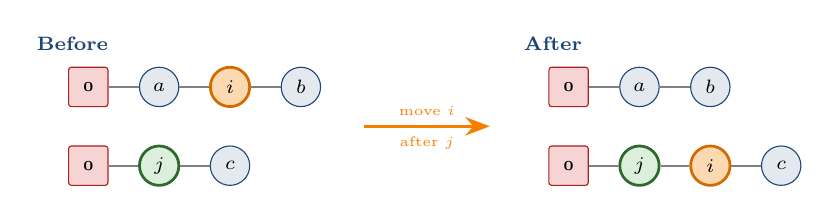
\begin{tikzpicture}[>=Stealth,
      nd/.style ={circle, draw=darkblue, fill=darkblue!12,
                  minimum size=0.5cm, inner sep=0pt, font=\scriptsize},
      dep/.style={draw=myred!80!black, fill=myred!20, rounded corners=1pt,
                  minimum size=0.5cm, inner sep=0pt, font=\tiny\bfseries},
      ii/.style ={circle, draw=myorange!85!black, fill=myorange!30, line width=1pt,
                  minimum size=0.5cm, inner sep=0pt, font=\scriptsize\bfseries},
      jj/.style ={circle, draw=mygreen!60!black, fill=mygreen!20, line width=1pt,
                  minimum size=0.5cm, inner sep=0pt, font=\scriptsize\bfseries},
      rt/.style ={thick, gray}]

    % ── BEFORE ──────────────────────────────────────────────
    \node[font=\scriptsize\bfseries, darkblue] at (-1.0,1.55) {Before};
    % route A
    \node[dep](a0) at (-0.8,1.0){0}; \node[nd](aa) at (0.1,1.0){$a$};
    \node[ii] (ai) at (1.0,1.0){$i$}; \node[nd](ab) at (1.9,1.0){$b$};
    \draw[rt] (a0)--(aa)--(ai)--(ab);
    % route B
    \node[dep](b0) at (-0.8,0.0){0}; \node[jj](bj) at (0.1,0.0){$j$};
    \node[nd] (bc) at (1.0,0.0){$c$};
    \draw[rt] (b0)--(bj)--(bc);

    % ── ARROW ───────────────────────────────────────────────
    \draw[->, line width=1.3pt, myorange]
      (2.7,0.5) -- node[above, font=\tiny]{move $i$}
                   node[below, font=\tiny]{after $j$} (4.3,0.5);

    % ── AFTER ───────────────────────────────────────────────
    \node[font=\scriptsize\bfseries, darkblue] at (5.1,1.55) {After};
    % route A (i removed)
    \node[dep](c0) at (5.3,1.0){0}; \node[nd](ca) at (6.2,1.0){$a$};
    \node[nd] (cb) at (7.1,1.0){$b$};
    \draw[rt] (c0)--(ca)--(cb);
    % route B (i inserted after j)
    \node[dep](d0) at (5.3,0.0){0}; \node[jj](dj) at (6.2,0.0){$j$};
    \node[ii] (di) at (7.1,0.0){$i$}; \node[nd](dc) at (8.0,0.0){$c$};
    \draw[rt] (d0)--(dj)--(di)--(dc);
  \end{tikzpicture}
  \end{center}
  \vspace{0.2em}
  \begin{center}\small
    \emph{We fix \highlight{insertion}: best fit with capacity --- many feasible \emph{inter-route} moves.}
  \end{center}
\end{frame}

% ──────────────────────────────────────────────────────────────────────────────
% Slide — Ensuring feasible neighbors (results removed)
% Say: many actions on a CVRP solution produce infeasible neighbors,
% typically capacity violations. We tested three feasibility strategies.
% Say (proactive masking, ours): we exploit the conditional pair selection.
% Pick the first node i freely from all customers (no capacity test yet).
% Then knowing i, compute the feasible partners and restrict π_θ to that
% subset for j. O(N) feasibility checks per step, not O(N^2).
% Say: proactive masking wins clearly; it is the key methodological
% extension over Neural SA.
% ──────────────────────────────────────────────────────────────────────────────
\begin{frame}{Ensuring Feasible Neighbors}
  \begin{block}{Proactive masking (ours)}
    \small Reuse the conditional sampling:\\[0.2em]
    \begin{itemize}\itemsep1pt
      \item Pick $i$ \emph{freely} from $\mathcal{C}$ -- no capacity check.
      \item Knowing $i$, compute feasible partners
            $\mathcal{A}_f(s,i) = \{ j : H(s,(i,j)) \in \mathcal{F} \}$
            and restrict $\pi_\theta(\cdot \mid s, i)$ to it.
    \end{itemize}
    \emph{Only $O(N)$ feasibility checks per step.}
  \end{block}
  \vspace{0.3em}
  \begin{block}{Alternatives we tested}
    \small
    \begin{itemize}\itemsep1pt
      \item \textbf{Reactive rejection:} sample any $a$, reject if
            infeasible. Cheapest per step; weakest learning signal.
      \item \textbf{Indirect rep.:} policy on customer permutations,
            greedy split rebuilds feasible routes. Always feasible but
            $\sim$4$\times$ slower per step.
    \end{itemize}
  \end{block}
\end{frame}

% ──────────────────────────────────────────────────────────────────────────────
% Slide — Input features
% Say: each node carries a local feature vector grouped into three
% categories — spatial, capacity, and search-state. These features are
% LOCAL: there is no fixed-size global descriptor, which is what makes
% the model scale-invariant.
% Note: the SA temperature and remaining-steps features let the policy
% adapt its behaviour to where we are in the schedule.
% ──────────────────────────────────────────────────────────────────────────────
\begin{frame}{Input Features: What the Policy Sees}
  \begin{columns}[T]
%    % ── Drawing: features belong to ONE node, every node has them ──────
%    \column{0.26\textwidth}
%    \begin{center}
%    \begin{tikzpicture}[>=Stealth, font=\tiny,
%        nd/.style ={circle, draw=darkblue, fill=darkblue!12,
%                    minimum size=0.38cm, inner sep=0pt},
%        ndi/.style={circle, draw=myorange!85!black, fill=myorange!30, line width=1pt,
%                    minimum size=0.42cm, inner sep=0pt, font=\tiny\bfseries}]
%      \node[nd] (q1) at (0,1.55){};
%      \node[ndi](qi) at (0.85,1.85){$i$};
%      \node[nd] (q3) at (1.6,1.5){};
%      \node[nd] (q4) at (0.6,1.0){};
%      \draw[gray, thick] (q4)--(q1)--(qi)--(q3);
%      % feature vector for node i
%      \node[draw=mypurple!70!black, fill=mypurple!10, rounded corners=2pt,
%            minimum width=0.7cm, minimum height=1.0cm] (fv) at (0.85,0.05){};
%      \foreach \yy in {0.34,0.17,0.0,-0.17,-0.34}
%        \draw[mypurple!70!black] (0.58,\yy)--(1.12,\yy);
%      \node[font=\tiny] at (0.85,-0.75){$\mathbf{x}_i$};
%      \draw[->, myorange, thick] (qi) -- (fv.north);
%    \end{tikzpicture}
%    \end{center}
%    {\centering\tiny Every node $i$ carries the \highlight{same} vector $\mathbf{x}_i$
%     --- all \highlight{standardized}.\par}
%
    % ── Three feature groups ──────────────────────────────────────────
    \column{0.29\textwidth}
    \begin{block}{Spatial}
      \small
      \begin{itemize}\itemsep1pt
        \item Coords, depot
        \item Route neighbors
        \item Angle, radial dist.
      \end{itemize}
    \end{block}

    \column{0.29\textwidth}
    \begin{block}{Capacity}
      \small
      \begin{itemize}\itemsep1pt
        \item Demand $q_i/Q$
        \item Route load
        \item Slack, depot flag
      \end{itemize}
    \end{block}

    \column{0.29\textwidth}
    \begin{block}{Search}
      \small
      \begin{itemize}\itemsep1pt
        \item Temperature $T$
        \item Remaining steps
      \end{itemize}
    \end{block}
  \end{columns}
  \vspace{0.7em}
  \begin{itemize}\small
    \item[] Local, node-centric encoding $\Rightarrow$ \highlight{scale-invariant}:
    \emph{same model from small to large $N$, no retraining.}
    \end{itemize}
        % ── Drawing: features belong to ONE node, every node has them ──────
%    \column{0.26\textwidth}
\vspace{-1em}
    \begin{center}
    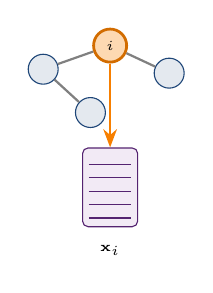
\begin{tikzpicture}[>=Stealth, font=\tiny,
        nd/.style ={circle, draw=darkblue, fill=darkblue!12,
                    minimum size=0.38cm, inner sep=0pt},
        ndi/.style={circle, draw=myorange!85!black, fill=myorange!30, line width=1pt,
                    minimum size=0.42cm, inner sep=0pt, font=\tiny\bfseries}]
      \node[nd] (q1) at (0,1.55){};
      \node[ndi](qi) at (0.85,1.85){$i$};
      \node[nd] (q3) at (1.6,1.5){};
      \node[nd] (q4) at (0.6,1.0){};
      \draw[gray, thick] (q4)--(q1)--(qi)--(q3);
      % feature vector for node i
      \node[draw=mypurple!70!black, fill=mypurple!10, rounded corners=2pt,
            minimum width=0.7cm, minimum height=1.0cm] (fv) at (0.85,0.05){};
      \foreach \yy in {0.34,0.17,0.0,-0.17,-0.34}
        \draw[mypurple!70!black] (0.58,\yy)--(1.12,\yy);
      \node[font=\tiny] at (0.85,-0.75){$\mathbf{x}_i$};
      \draw[->, myorange, thick] (qi) -- (fv.north);
    \end{tikzpicture}
    \end{center}
    \vspace{-1em}
    {\centering\scriptsize Every node $i$ carries the \highlight{same} vector $\mathbf{x}_i$
     --- all \highlight{standardized}.\par}

\end{frame}

% ──────────────────────────────────────────────────────────────────────────────
% Slide — SA on CVRP as an MDP + PPO
% Say: To bring in RL, we frame the SA loop as a Markov Decision Process.
% State = full feasible solution; action = node pair (i,j); reward = tiered
% (penalty if infeasible, 0 if rejected, normalised ΔC if accepted).
% Say: we train the policy with PPO — a standard on-policy gradient method
% (Schulman et al., 2017). Actor outputs the action distribution; critic
% estimates the value. PPO is not a contribution of this work; we use it
% off-the-shelf.
% ──────────────────────────────────────────────────────────────────────────────
%\begin{frame}{Framing SA as a Markov Decision Process}
\begin{frame}{Training LG-SA with Proximal Policy Optimization (PPO)}
  \begin{columns}[T]
    \column{0.63\textwidth}
    \small We frame LG-SA as an \highlight{MDP} $\Rightarrow$ train with \highlight{PPO}. \smallskip
    
    \begin{block}{State $s_t$}
      \small Per-node features of the current feasible solution.
    \end{block}
    \vspace{0.1em}
    \begin{block}{Action $a_t$}
      \small Node pair $(i, j)$ for operator $H$.
    \end{block}
    \vspace{0.1em}
    \begin{block}{Reward $r_t$ -- the one that works}
      \small We tested several classic RL rewards. Best: the
      \highlight{score difference} old $\to$ new solution ($+$ or $-$).\\[0.2em]
      \emph{$=0$ on steps where SA rejects the move.}
    \end{block}

    \column{0.35\textwidth}
    \vspace{0.2em}
%    \begin{center}
%    \begin{tikzpicture}[>=Stealth, thick,
%        every node/.style={font=\scriptsize},
%        sB/.style={draw=darkblue, fill=darkblue!15, rounded corners=2pt,
%                   inner sep=2pt, minimum height=0.5cm, font=\scriptsize},
%        aB/.style={draw=myorange!80!black, fill=myorange!15, rounded corners=2pt,
%                   inner sep=2pt, minimum height=0.5cm, font=\scriptsize}]
%      % Row 1
%      \node[sB] (s0) {$s_t$};
%      \node[aB, right=0.45cm of s0] (a0) {$a_t$};
%      \node[sB, right=0.55cm of a0] (s1) {$s_{t+1}$};
%      % Row 2
%      \node[aB, below=0.55cm of s1] (a1) {$a_{t+1}$};
%      \node[sB, left=0.55cm of a1] (s2) {$s_{t+2}$};
%      \node[left=0.35cm of s2] (dots) {$\cdots$};
%
%      % Arrows row 1
%      \draw[arr] (s0) -- node[above, font=\tiny]{$\pi_\theta$} (a0);
%      \draw[arr] (a0) -- node[above, font=\tiny]{$P$}
%                        node[below, font=\tiny]{$r_t$} (s1);
%      % Wrap to row 2
%      \draw[arr] (s1.east) -- ++(0.18,0) |- (a1.east);
%      \node[font=\tiny] at ($(s1.east)+(0.42,-0.28)$) {$\pi_\theta$};
%      % Arrows row 2 (right to left)
%      \draw[arr] (a1) -- node[above, font=\tiny]{$P$}
%                        node[below, font=\tiny]{$r_{t+1}$} (s2);
%      \draw[arr] (s2) -- (dots);
%
%      % PPO container
%      \begin{scope}[on background layer]
%        \node[draw=mypurple!70!black, fill=mypurple!8,
%              rounded corners=5pt, line width=1pt,
%              fit=(s0)(a0)(s1)(a1)(s2)(dots),
%              inner xsep=8pt, inner ysep=10pt] (ppo) {};
%      \end{scope}
%      \node[anchor=north west, font=\scriptsize\bfseries,
%            text=mypurple!70!black]
%            at ([xshift=4pt,yshift=-2pt]ppo.north west) {PPO};
%    \end{tikzpicture}
%    \end{center}

\begin{figure}[h!]
\begin{center}
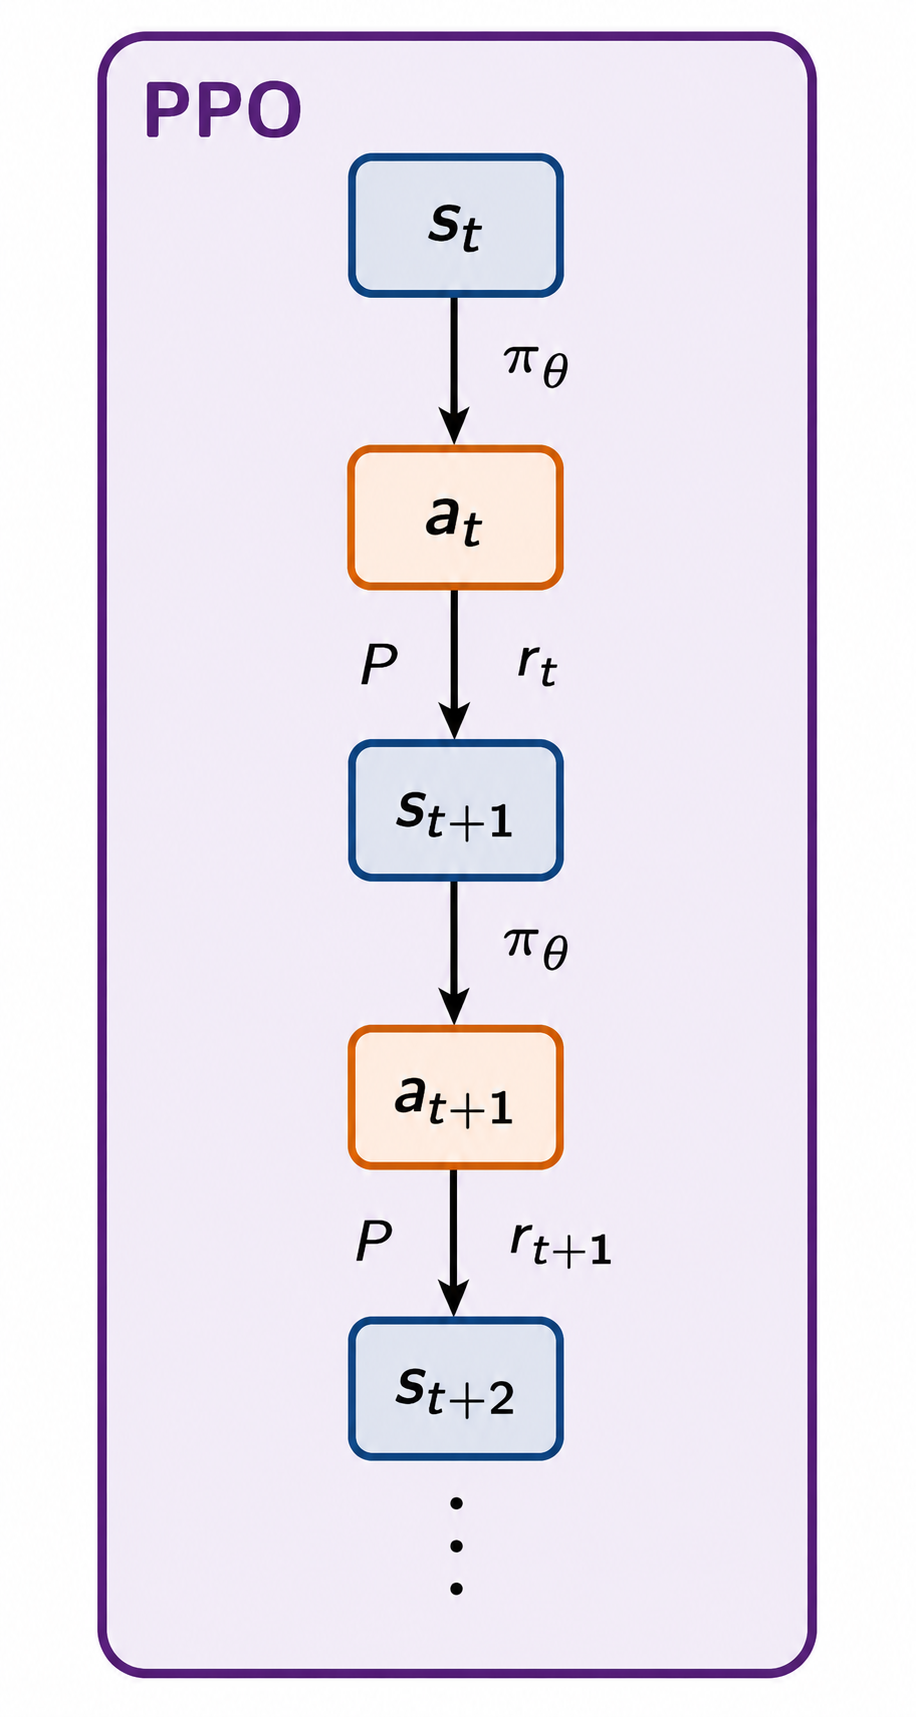
\includegraphics[height=5.7cm]{figures/PPO.png}
%\caption{default}
\label{default}
\end{center}
\end{figure}

\begin{center}\scriptsize
\emph{PPO} [Schulman et al., 2017]\\
actor $\pi_\theta$ \,+\, critic $V_\phi$\\ (standard, off-the-shelf)
\end{center}
\end{columns}
\end{frame}

% ══════════════════════════════════════════════════════════════════════════════
\section{Design Choices}
% ══════════════════════════════════════════════════════════════════════════════

% ──────────────────────────────────────────────────────────────────────────────
% Slide — Design choices that matter (NO costs; qualitative)
% Say (test set): all parameter studies use 10,000 CVRP instances at N=100
% sampled uniformly in [0,1]^2 with demands in {1..9} — the standard
% Nazari distribution. 10k SA steps per instance, run in parallel on one GPU.
%
% Say (greedy vs sampling): the policy outputs a softmax. Standard RL at
% inference picks the arg-max — always the top-scored node. We do the
% opposite: we SAMPLE. So we usually pick a high-scored node, but not
% always the top one — that injected randomness is exactly the diversity
% SA needs. Greedy = always best score → search collapses. (We checked:
% greedy degrades by a wide margin across all configurations.)
%
% Say (training init): we train with a mix of initialisations (random,
% nearest neighbour, sweep, isolate). Multi-init is the most robust;
% nearest-neighbour init alone traps the policy in deep local optima.
%
% Say (testing init): once trained, the policy converges to nearly the
% same final cost whatever initial solution we hand it — it has learned a
% global reorganisation, not a local repair.
%
% Say (cross-domain): training on the harder Queiroga distribution
% generalises to the simpler Nazari one. The reverse does not hold —
% training on uniform Nazari is too easy a curriculum.
%
% Say (Metropolis): even WITH the learned policy, keeping the Metropolis
% acceptance criterion improves results across ALL feasibility strategies.
% The policy is a smarter proposer, not a replacement for SA's
% explore/exploit balance.
% ──────────────────────────────────────────────────────────────────────────────
%\begin{frame}{Design Choices that Matter}
%  \begin{itemize}\small
%  \item[] The method is \highlight{simple} --- but a few choices are \bad{not optional}: \emph{remove any one and it stops working.}
%  \end{itemize}
%  %\vspace{0.2em}
%
%  \begin{columns}[T]
%    \column{0.53\textwidth}
%    \begin{block}{Sample, never arg-max}
%      \small Sample from the softmax at inference. Greedy collapses
%      the search; sampling gives SA the diversity it needs.
%    \end{block}
%    \vspace{0.3em}
%    \begin{block}{Keep Metropolis}
%      \small Even with the learned policy, the SA acceptance rule
%      still helps. The policy is a smarter proposer -- not a replacement.
%    \end{block}
%
%    \column{0.4\textwidth}
%    \begin{block}{Multi-init training}
%      \small Mix random / NN / sweep / isolate per episode.
%      A single init (esp.\ nearest-neighbour) traps the policy in deep
%      local optima.
%    \end{block}
%    %\vspace{0.1em}
%    \begin{block}{Feature choice matters}
%      \small The features are few but \highlight{carefully chosen}:
%      drop a single one and quality drops \bad{sharply}.
%    \end{block}
%  \end{columns}
%
%  \vspace{0.3em}
%  \begin{center}\small
%    \emph{Once trained, the policy reaches the same quality from any starting solution.}
%  \end{center}
%\end{frame}


\begin{frame}{Design Choices that Matter}
\small

\begin{itemize}
\item[] The method is \highlight{simple} --- but a few choices are \bad{not optional}: \emph{remove any one and it stops working.}
\end{itemize}

\begin{block}{}
\begin{itemize}
\item \small{\bf Sample, never arg-max:} 
Sample from the softmax at inference. \\ \smallskip
\footnotesize{Greedy collapses the search; sampling gives SA the diversity it needs.} \smallskip
\item \small{\bf Keep Metropolis:} 
Even with learned policy, SA acceptance rule helps. \\ \smallskip
\footnotesize{The policy is a smarter proposer -- not a replacement.}
\smallskip
\item \small{\bf Multi-init training:} 
Mix random / NN / sweep / isolate per episode. \\ \smallskip
\footnotesize{A single init (esp.\ NN) traps the policy in deep local optima.}
\smallskip
\item \small{\bf Feature choice matters:} 
The features are few but \highlight{carefully chosen}. \\ \smallskip
\footnotesize{Drop a single one and quality drops \bad{sharply}.}
\end{itemize}
\end{block}

\begin{itemize}
\item[] \emph{Once trained, the policy reaches the same quality from any starting solution.}
\end{itemize}

\end{frame}

% ══════════════════════════════════════════════════════════════════════════════
\section{Results}
% ══════════════════════════════════════════════════════════════════════════════

% ──────────────────────────────────────────────────────────────────────────────
% Slide — SA vs LG-SA (the core comparison): cost vs steps
% Say (enthusiastic): this is the heart of the story. Blind SA plateaus high
% even with a huge step budget. Guidance reaches in a FRACTION of the steps
% what blind SA never reaches. The guidance does the work. Don't read numbers.
% ──────────────────────────────────────────────────────────────────────────────
\begin{frame}{SA vs.\ LG-SA: Guidance Does the Work}
  \begin{columns}[T]
    \column{0.50\textwidth}
    \vspace{0.4em}
    \begin{center}
    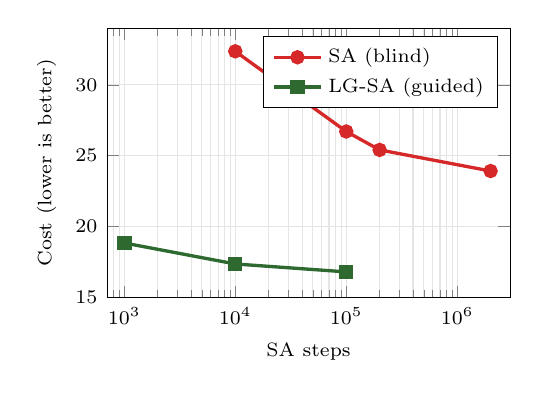
\begin{tikzpicture}
    \begin{axis}[
        width=6.7cm, height=5cm,
        xmode=log, log basis x=10,
        xlabel={SA steps}, ylabel={Cost (lower is better)},
        xlabel style={font=\scriptsize}, ylabel style={font=\scriptsize},
        tick label style={font=\scriptsize},
        xmin=700, xmax=3e6, ymin=15, ymax=34,
        grid=both, grid style={gray!20},
        legend style={font=\scriptsize, at={(0.97,0.97)}, anchor=north east},
        legend cell align=left,
      ]
      % blind SA (no policy)
      \addplot[myred, very thick, mark=*, mark options={fill=myred}]
        coordinates {(1e4,32.37) (1e5,26.71) (2e5,25.41) (2e6,23.92)};
      \addlegendentry{SA (blind)}
      % LG-SA
      \addplot[mygreen!60!black, very thick, mark=square*, mark options={fill=mygreen!60!black}]
        coordinates {(1e3,18.84) (1e4,17.36) (1e5,16.80)};
      \addlegendentry{LG-SA (guided)}
    \end{axis}
    \end{tikzpicture}
    \end{center}

    \column{0.42\textwidth}
    \vspace{0.2em}
    \begin{alertblock}{The guidance does the work}
      \footnotesize
      \begin{itemize}\itemsep4pt
        \item Blind SA \bad{plateaus high} --- even with a huge step budget
        \item Guided SA reaches \good{far lower cost} in a \good{fraction of the steps}
        \item Same loop, same operator --- \highlight{only the proposal changed}
      \end{itemize}
    \end{alertblock}
  \end{columns}
\end{frame}

% ──────────────────────────────────────────────────────────────────────────────
% Slide — LG-SA vs classical & learning baselines (N=100), combined
% Say (enthusiastic, NO numbers): a tiny model lands right in the sweet spot.
% It matches strong classical and neural methods in cost, while being far
% faster than the heavy improvement learners — and it scales.
% ──────────────────────────────────────────────────────────────────────────────
\begin{frame}{LG-SA vs.\ Classical \& Learning Baselines ($N=100$)}
  \begin{columns}[T]
    \column{0.5\textwidth}
    \footnotesize
    \setlength{\tabcolsep}{3pt}
    \begin{tabular}{lrr}
      \toprule
      Method & Cost & Time \\
      \midrule
      \textit{Classical} & & \\
      LKH3                       & 15.65 & 13\,h \\
      OR-Tools                   & 16.61 & 29\,m \\
      \midrule
      \textit{Learning} & & \\
      NLNS~{\tiny[Hottung \& Tierney, 2022]}     & 15.99 & 1\,h\,02\,m \\
      LIH~{\tiny[Wu et al., 2022]}               & 16.03 & 5\,h \\
      CDCP~{\tiny[Garc\'ia-Torres et al., 2022]} & 15.85 & 19\,h \\
      \midrule
      \textit{Ours} & & \\
      \rowcolor{myorange!30}
      LG-SA ($10^5$) & \good{16.80} & \good{29\,m} \\
      \bottomrule
    \end{tabular}

    \column{0.42\textwidth}
    \vspace{0.6em}
    \begin{alertblock}{A tiny model \scriptsize{(in the sweet spot)}}
      \small
      \begin{itemize}\itemsep3pt
        \item \good{Matches} strong classical \& neural methods in cost
        \item \good{Far faster} than the heavy improvement learners
        \item And it \highlight{scales} to large $N$ with no retraining
      \end{itemize}
    \end{alertblock}
  \end{columns}
\end{frame}

% ══════════════════════════════════════════════════════════════════════════════
\section{Conclusion}
% ══════════════════════════════════════════════════════════════════════════════

% ──────────────────────────────────────────────────────────────────────────────
% Slide — Conclusion
% Say: LG-SA is PPO-guided simulated annealing for CVRP. Key methodological
% pieces: proactive masking for feasibility, conditional architecture
% scaling linearly, and stochastic sampling at inference. 42% improvement
% over classical SA and competitive against state-of-the-art neural methods.
% Note (ongoing): same LG-SA backbone with curriculum training and a few
% training-side tricks now matches SOTA construction AND improvement
% learning methods at N=100 in both cost and execution time. Next paper.
% ──────────────────────────────────────────────────────────────────────────────
\begin{frame}{Conclusion \& Ongoing Work}
  \begin{columns}[T]
    \column{0.57\textwidth}
    \begin{block}{Contributions}
      \small
      \begin{itemize}\itemsep2pt
        \item \good{LG-SA:} PPO-guided SA that brings DRL to CVRP
        \item \good{Proactive masking:} the key that makes feasibility work
        \item \good{Conditional policy:} $O(N)$ action space
        \item \good{Scalability:} one model, $N=50 \to 1000$, no retraining
      \end{itemize}
    \end{block}
    \vspace{0.3em}
    \begin{exampleblock}{Ongoing work}
      \small Same LG-SA backbone $+$ \textbf{curriculum training} and training-side tricks%: now \emph{matches SOTA construction \& improvement} learning methods at $N{=}100$ in both cost and time.
    \end{exampleblock}

    \column{0.38\textwidth}
    \begin{alertblock}{Future directions}
      \small
      \begin{enumerate}\itemsep2pt
        \item LNS operators (destroy \& repair)
        \item GNN encoder for global context
        \item Rich VRP variants (TW, multi-depot)
      \end{enumerate}
    \end{alertblock}
    \vspace{1.5em}
    \begin{center}
      \Large\textbf{Thank you!}\\[0.4em]
      \normalsize\texttt{jules.andretti@uvsq.fr}
    \end{center}
  \end{columns}
\end{frame}

\end{document}
